
\section{\uppercase{Twitter LDA}}
An issue pertaining to the use of LDA on Twitter data is the questionable assumption of considering a tweet as a mixture of topics. Given the extremely short nature of tweets, most tweets consists of a single topic. As discussed above, some studies have tackled this problem by aggregating the tweets of a user in a single document. This method, though effective, is not guarenteed to help much because of the fact that users generally express a wide variety of different topics in their tweets which may not be related to each other. This analysis will still be good if we want to profile users; but since our aim is to mine events from the topics, the possible solutions that seems feasible will be to aggregate tweets based on time, locality and hashtags.

To this end, \cite{zhao2011comparing} have proposed an effective variant of the standard LDA, called Twitter LDA. It is based on the assumption that a tweet will contain a single topic chosen from a topic distribution of a particular user. 

\subsection{Model Description} 
The generative model makes the following assumptions. Twitter data has T number of topics. When a user wants to write a tweet, he/she selects a topic from his/her favourite list of topics, these topics will be from the T topics. Then for the selected topic, the user selects a bag of words, one by one from the distibution of words over topics. However not all words of a tweet are closely related the topic. Many of them are just common words occuring in tweets of various different topics. So for each words user decides whether it is a background word or a topic word and then chooses the word from its respective distribution.
 \begin{figure*}
 \centering
 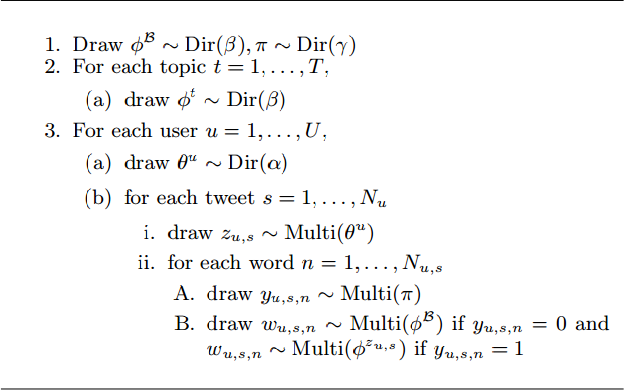
\includegraphics[width=0.6\textwidth]{figures/lda-algo}
 \caption{Twitter LDA Generative Process}
 \label{fig:twitterlda-algo}
\end{figure*}

Formally, let $\theta_u$ denotes the topic distribution for a user $u$. Let $\phi_t$ be the distribution of words for the topic $t$ and let $\phi_B$ be the distribution of background words. $\pi$ is a bernouli distribution which denote the choice of a word to be a background or a topic word. $\alpha~\beta~\gamma$ are dirichlet parameter used for generating respective dirichlet distributions. The plate notation for the model is given in figure \ref{fig:plate} The generative algorithm is given in figure \ref{fig:twitterlda-algo}.